\documentclass{jib}
\newlength{\platz}
\setlength{\platz}{15pt}
\RequirePackage{listings}

\usepackage{changepage} %test, TODO remove

\lstset{%
  basicstyle=\ttfamily,
  fontadjust,
  flexiblecolumns=true,
  frame=L,
  xleftmargin=15pt,
  framesep=5pt,
  emphstyle=\rmfamily\itshape}
  

%%%%%%%%%%%%%%%%%%%%%%%%%%%%%%%%%%%%%%%%%%%%%%%%%%%%%%%%%%
% JIB Header/Footer
%%%%%%%%%%%%%%%%%%%%%%%%%%%%%%%%%%%%%%%%%%%%%%%%%%%%%%%%%%
%\jibvolume{XX} % insert volume
%\jibissue{X}   % insert issue
%\jibpages{XXX} % insert article ID
%\jibyear{XXXX} % insert year
%\makeHeaderFooter{} % leave as is
%%%%%%%%%%%%%%%%%%%%%%%%%%%%%%%%%%%%%%%%%%%%%%%%%%%%%%%%%%

\begin{document}

%%%%%%%%%%%%%%%%%%%%%%%%%%%%%%%%%%%%%%%%%%%%%%%%%%%%%%%%%%
%
% Title Page
%
%%%%%%%%%%%%%%%%%%%%%%%%%%%%%%%%%%%%%%%%%%%%%%%%%%%%%%%%%%

\begin{jibtitlepage}

\jibtitle{Description of the \LaTeX\ style files for the
Journal of Integrative Bioinformatics (version 7.2017)}


%We did not provide author(s) nor author footnote(s), please complete as applicable.
% Please make sure to use unique footnote characters for each author
\jibauthor{Firstname Lastname\iref{imbio},
           Firstname Lastname\iref{imbio},
           Firstname Lastname\iref[,]{imbio}\jibauthorfootnote{*}{To whom
           correspondence should be addressed. Email:
           \email{jib.editorial@degruyter.de}}}

\addjibinstitution{imbio}{IMBio, Ralf Hofest\"adt, Bielefeld University, Faculty
of Technology, Bioinformatics Department, D-33501 Bielefeld, Germany,
\url{http://www.imbio.de}}

\end{jibtitlepage}


% \begin{abstract}
% 
% This document is a short description of the \LaTeX\ \emph{document class} \emph{jib} and its use. It shall be used to submit \LaTeX\ articles to the \emph{Journal of Integrative Bioinformatics} and at the same time may be used to check whether your \LaTeX\ installation can compile output files according to the guidelines of the journal.
% 
% \end{abstract}

% adjusts the width of the abstract, please do not change!
\begin{adjustwidth}{}{1cm}                 

\abstract{This document is a short description of the \LaTeX\ \emph{document class} \emph{jib} and its use. It shall be used to submit \LaTeX\ articles to the \emph{Journal of Integrative Bioinformatics} and at the same time may be used to check whether your \LaTeX\ installation can compile output files according to the guidelines of the journal.
}

\end{adjustwidth} % please sdo not change

\textbf{Keywords:} Keyword 1, Keyword 2, Keyword 3, Keyword 4, Keyword 5 

%%%%%%%%%%%%%%%%%%%%%%%%%%%%%%%%%%%%%%%%%%%%%%%%%%%%%%%%%%
%
% Manuscript Content
%
%%%%%%%%%%%%%%%%%%%%%%%%%%%%%%%%%%%%%%%%%%%%%%%%%%%%%%%%%%


%%%%%%%%%%%%%%%%%%%%%%%%%%%%%%%%%%%%%%%%%%%%%%%%%%%%%%%%%%
%
% Introduction 
%
%%%%%%%%%%%%%%%%%%%%%%%%%%%%%%%%%%%%%%%%%%%%%%%%%%%%%%%%%%

\section{Introduction}

This text is based on the original Instruction for Authors. The most-recent
version of the Instructions for Authors are available from:
\url{https://www.degruyter.com/view/j/jib}

\subsection{Aims and Scope} 
The Journal of Integrative Bioinformatics (JIB) is an
international open access journal publishing original peer-reviewed research
articles in all aspects of integrative bioinformatics.
This includes: molecular databases, information systems and data warehouses,
integration of data (methods and tools), metabolic and regulatory network
modeling and simulation, signal pathways and cell control, network analysis,
medical informatics, biomedicine and biotechnology, integrative approaches for
drug design as well as integrative data and text mining approaches.
The journal will only accept papers which present new tools or new aspects of
already JIB published tools. Furthermore, these tools must be available and
usable via the internet and free of charge for academicians. For accepted review
publications you are invited to join JIBtools as an editor for a new topic:
\url{http://imbio.de/journal/JIBtools}


\subsection{Editorial Policy}

Manuscripts are independently reviewed by peers selected by the Editors.
Decisions are reached as quickly as possible. JIB aspires to notify authors
within 6 weeks from submission date. When manuscripts are accepted subject to
revision, the revised manuscript should be returned within 6 weeks. Accepted
papers are promptly published online as soon as they have been finally
processed.


\subsubsection{Authorship}

Authorship is restricted to those who have made a significant contribution to
the conceptual design of the study and/or the execution of the study.


\subsubsection{Unpublished Material} 

Submission of a manuscript to JIB implies that the work described is not
copyrighted, published or submitted elsewhere, except in abstract form. The
corresponding author should ensure that all authors approve the manuscript
before its submission to JIB.


\subsubsection{Ethical conduct of research} 

The authors must describe and confirm safeguards to meet ethical standards. The
ethics statements for the Journal of Integrative Bioinformatics are based on the
Committee on Publication Ethics (COPE) Best Practice Guidelines for Journal
Editors (see \url{http://publicationethics.org}) and the ``Uniform Requirements
for Manuscripts (URM) Submitted to Biomedical Journals'' of the International
Committee of Medical Journal Editors (ICMJE – \url{http://www.icmje.org}).
Where applicable, all authors must confirm in writing that they have complied
with the World Medical Association Declaration of Helsinki (see
\url{http://www.wma.net/en/30publications/10policies/b3/}) regarding ethical
conduct of research involving human subjects. In the Materials and Methods
Section, or in a separate section, the manuscript should contain a statement
that the study has been approved by the Ethical Committee of the institution
where the study was performed, and that the study subjects, or their legal
guardians, gave informed consent for participation in the study. If preclinical
studies performed with animals are described, authors must confirm in writing
that institutional and national standards for the care and use of laboratory
animals were followed (please consult the International Association of
Veterinary Editors' Consensus Author Guidelines on Animal Ethics and Welfare for
further guidance).
Please also note that JIB uses the plagiarism detection software “iThenticate”
to check for potential overlaps with prior publications. Any previously
published material must be referenced appropriately in the manuscript.


\subsubsection{Conflict of Interest} 

When authors submit a manuscript, they are responsible for recognizing and
disclosing financial and/or other conflicts of interest that might bias their
work and/or could inappropriately influence his/her judgment. Upon submission,
the author(s) will be required to complete a form to declare any conflicts of
interest, funding, employment, or leadership and honoraria. This information
must also be included within the manuscript before the Reference section. Please
consult our Publication Ethics and Malpractice Statement first; if you do not
have any conflicts of interest to report, insert the following declaration:
Conflict of interest statement: Authors state no conflict of interest. All
authors have read the journal's publication ethics and publication malpractice
statement available at the journal's website and hereby confirm that they comply
with all its parts applicable to the present scientific work.
If no specified acknowledgement is given, the Publishers assume that no conflict
of interest exists.


\subsubsection{Manuscript Submission} 

Manuscripts should be submitted in
electronic form to our online submission, peer review and production system at
\url{http://mc.manuscriptcentral.com/dgjib}.


\subsection{Preparation of Manuscript}

\subsubsection{Language}

Manuscripts should be written in clear and concise English. Please have your
text proofread by an English native speaker before you submit it for
consideration. At the proof stage, only minor changes other than corrections of
printers' errors are allowed.

\subsubsection{Cover Letter}

Each manuscript should be accompanied by a cover letter containing a brief
statement by the authors describing the novelty and importance of their
research.

\subsubsection{Nomenclature}

Authors are asked to follow the recommendations of the
Syst\`eme International d'Unit\'es (SI):
\url{http://www.bipm.org/en/publications/si-brochure/}

\subsubsection{General format}

Manuscripts (including tables and figures, table and figure legends, and
references) should be typed double- spaced with font size 12 letters. Pages
should be numbered and have margins of 2.5 cm (1 inch) on all sides. Please
avoid footnotes in the text, use parentheses instead.

\subsubsection{Article types}

JIB welcomes research articles, review papers and workshop contributions within
the scope of the journal. If you submit a workshop contribution you will be
asked to further classify your submission.

\subsubsection{General structure of the text body}

Original research articles should be organized into: Title page, Abstract,
Keywords, List of non-standard abbreviations (if applicable), Introduction,
Related works, Architecture/Implementation/Workflow, Application, Discussion,
Acknowledgments (if applicable), Conflict of Interest statement, References,
Tables and Figures legends.

Review articles should include: Title page, Abstract, Keywords, Body with
subsections, Acknowledgments (if applicable), Conflict of Interest statement,
and References.

\subsubsection{Abstract and Keywords}

The first page of the manuscript should contain the Abstract and the Keywords.
The Abstract should be a single paragraph of not more than 200 words (original
article or review) which must be comprehensible to readers before they have read
the paper. Below the Abstract, up to five keywords, which are not part of the
title, should be given in alphabetical order and separated by semicolons.

\subsubsection{Abbreviations, Variables, Quotations and more \ldots}

Standard abbreviations in the field of Integrative Bioinformatics do not
necessarily have to be introduced. If you introduce new abbreviations, please
write them at the first occurrence in italic, like Integrative Bioinformatics
(IB), and then in the following text just use the abbreviation in standard font.
Also, special or Latin terms in the text should be written in italic i.
For quotations, please indicate them like this: ``The 2nd prize was awarded to''
(1). Please also note the writing of the ordinal number: ``2nd''.

\subsubsection{References}

Reference lists have to be written in Vancouver style, please see:
\\
\url{http://guides.lib.monash.edu/citing-referencing/vancouver} 
\\
The names of journals should be abbreviated according to the World List of
Scientific Periodicals.
\\
Number the references consecutively in the order in which they appear in the
text, including tables and figures. In the body text, identify references by
Arabic numerals in round brackets (1). In the references all authors must be
included; et al. is not accepted. Do not use italic font in the reference
section.

\subsubsection{Tables}

Submit tables on separate pages and number them consecutively using Arabic
numerals. Provide a short descriptive title, column headings, and (if necessary)
footnotes to make each table self-explanatory. Refer to tables in the text as
Table 1, etc. Use Table 1, etc. in the table legends. Please indicate in the
manuscript the approximate position of each table.

\subsubsection{Figures}

Illustrations will be reduced in size to fit, whenever possible, the width of a
single column. Lettering in all figures within the article should be uniform in
style, preferably a sans serif typeface, and of sufficient size, so that it is
readable at the final size of approximately 2 mm. Uppercase letters A, B, C,
etc. should be used to identify parts of multi-part figures. Cite all figures in
the text in a numerical order. Indicate the approximate position of each figure.
Refer to figures in the text as Figure 1, etc. Use Figure 1, etc. in the figure
legends.
\\
Please note that if any of the figures you used are copyrighted, you need to
obtain permission from the copyright owners to reproduce these figures in JIB.
You also need to document the copyright permission in the respective figure
legend. The same holds true for copyrighted tables you use.

\subsubsection{Colour figures}

Authors are encouraged to submit illustrations in color if necessary for their
scientific content. Publication of color figures is provided free of charge both
in online and print editions. Line drawings and photographs must be of high
quality. Please note that faint shading may be lost upon reproduction.

\subsubsection{Figure legends}

Provide a short descriptive title, and (if necessary) footnotes to make each
figure self-explanatory on separate pages. Explain all symbols used in the
figures. Remember to use the same abbreviations as in the body-text.

\subsubsection{Note for authors of NIH-funded research}

Walter de Gruyter Publishers acknowledge that the author of an NIH-funded
article retains the right to provide a copy of the final manuscript to NIH upon
acceptance for publication or thereafter, for public archiving in PubMed Central
12 months after publication in JIB note that only the accepted author's version
of the manuscript, not the PDF file of the published article, may be used for
NIH archiving.

\subsection{Contact}

Please contact us for any further questions:

\subsubsection{Scientific contact:}

\email{jib.editorial@degruyter.com}
(JIB Editorial Office)

\subsubsection{Publisher contact:}

Alexandra Hinz, Journal Manager DE GRUYTER
\\
Genthiner Straße 13
\\
10785 Berlin, Germany
\\
Tel. +49-30-26005-358 / Fax: +49-30-26005-325
\\ 
E-mail:
\email{alexandra.hinz@degruyter.com}


%%%%%%%%%%%%%%%%%%%%%%%%%%%%%%%%%%%%%%%%%%%%%%%%%%%%%%%%%%
%
% Related works
%
%%%%%%%%%%%%%%%%%%%%%%%%%%%%%%%%%%%%%%%%%%%%%%%%%%%%%%%%%%
\section{Related works}

This is an example text for a section.

%%%%%%%%%%%%%%%%%%%%%%%%%%%%%%%%%%%%%%%%%%%%%%%%%%%%%%%%%%
%
% Architecture/Implementation
%
%%%%%%%%%%%%%%%%%%%%%%%%%%%%%%%%%%%%%%%%%%%%%%%%%%%%%%%%%%
\section{Architecture/Implementation/Workflow}

This is an example text for a section.

%%%%%%%%%%%%%%%%%%%%%%%%%%%%%%%%%%%%%%%%%%%%%%%%%%%%%%%%%%
%
% Application
%
%%%%%%%%%%%%%%%%%%%%%%%%%%%%%%%%%%%%%%%%%%%%%%%%%%%%%%%%%%
\section{Application}

This is an example text for a section.

%%%%%%%%%%%%%%%%%%%%%%%%%%%%%%%%%%%%%%%%%%%%%%%%%%%%%%%%%%
%
% Discussion
%
%%%%%%%%%%%%%%%%%%%%%%%%%%%%%%%%%%%%%%%%%%%%%%%%%%%%%%%%%%
\section{Discussion}

This is an example text for a section.


%%%%%%%%%%%%%%%%%%%%%%%%%%%%%%%%%%%%%%%%%%%%%%%%%%%%%%%%%%
%
% Acknowledgements
%
%%%%%%%%%%%%%%%%%%%%%%%%%%%%%%%%%%%%%%%%%%%%%%%%%%%%%%%%%%
\section*{Acknowledgements}
%
Place your acknowledgements here.
%


%%%%%%%%%%%%%%%%%%%%%%%%%%%%%%%%%%%%%%%%%%%%%%%%%%%%%%%%%%
%
% Conflict of Interest
%
%%%%%%%%%%%%%%%%%%%%%%%%%%%%%%%%%%%%%%%%%%%%%%%%%%%%%%%%%%
\section*{Conflict of interest statement}
%
Here you can state any conflicts of interest.
\\
Please consult our Publication Ethics and Malpractice Statement. If you do not
have any conflicts of interest to report, please use this text:
\\
``Conflict of interest statement: Authors state no conflict of interest. All
authors have read the journal's Publication ethics and publication malpractice
statement available at the journal's website and hereby confirm that they comply
with all its parts applicable to the present scientific work.''


%%%%%%%%%%%%%%%%%%%%%%%%%%%%%%%%%%%%%%%%%%%%%%%%%%%%%%%%%%
%
% LATEX Template Introduction 
%
%%%%%%%%%%%%%%%%%%%%%%%%%%%%%%%%%%%%%%%%%%%%%%%%%%%%%%%%%%
\section{\LaTeX\ Template Introduction}

The regular doecument ends with the Conflict of interest statement, followed by
the references (see bottom of this document). In this extra section, the \LaTeX\
 styles are discussed.

Please read these instructions carefully and follow them strictly so that the
publication process is efficient. The Journal of Integrative Bioinformatics
(JIB) reserves the right to return submissions that are not prepared in
accordance with the following instructions and layout guidelines.

In order to conform to the guidelines of JIB, the document class \emph{jib} has
to be used in the preamble of your \TeX-file.

\begin{lstlisting}
\documentclass{jib}
\end{lstlisting}

The document class \emph{jib} has been derived from the standard document class
\emph{article}. Thus, a runnable version of \LaTeX2e\ should be installed on
your system. The developed document class requires some \LaTeX\ packages that
are not included in a standard \LaTeX\ installation. Thus, it may then be
required to install the potentially missing packages.

In general, the contribution must be clearly structured. This is especially
important for long manuscripts. Any reasonable structure will be acceptable.
However, the following arrangement is recommended: Summary, Introduction,
Methods, Results, Discussion, References.

Please submit the complete \LaTeX\ source files (*.tex, *.bib, images) together
with a PDF version. PDF files for submission to the Journal of Integrative
Bioinformatics should be created using the following steps:

\begin{lstlisting}[emph={texfile,dvi,file}] first step:  latex texfile second
step: dvipdfm dvi-file
\end{lstlisting}

\subsection{Command Descriptions}

This section describes the various commands, their syntax and meaning.

\subsubsection{Title Page}

The title page has been defined as an environment. Thus, the special commands
that define the title page can only be used in this environment.

\begin{lstlisting}
\begin{jibtitlepage}
...
\end{jibtitlepage}
\end{lstlisting}

The title page contains the following three structures. The first
is the \emph{title} of the whole document. Second are the
\emph{authors} who contributed to the article. Third are
the \emph{institutions} the authors are affiliated with.

\subsubsection{Title Declaration}

\begin{lstlisting}[emph={title}]
\jibtitle{title}
\end{lstlisting}

The argument \emph{title} describes the title of the document.

\vspace{\platz}
\subsubsection{Author Declaration}

\begin{lstlisting}[emph={list, of, authors}]
\jibauthor{list of authors}
\end{lstlisting}

The argument \emph{list of authors} is the list of the manuscript's authors.
Usually it is a comma-separated list of the authors' names. Sometimes it is
necessary to place markings, that refer from an author to an institution.
Therefore, the \emph{iref}-statement should be used.

\begin{lstlisting}[emph={separator, label}]
\iref[separator]{label}
\end{lstlisting}

Only one reference can be specified with this statement. If more than one
reference should be added for an author, also more than one
\emph{iref}-statement has to be set. To define a reference, the label of that
institution has to be used. For constituting a label for an institution see
section \ref{sssec_inst_decl}. With the optional argument \emph{separator} a
separator symbol can be put to the actual reference, in case more than one
reference has been defined. Therefore, a comma should be used. The
\emph{default} value of this argument is \emph{no symbol}.

\begin{lstlisting}[emph={separator, marking, footnotetext}]
\jibauthorfootnote[separator]{marking}{footnotetext}
\end{lstlisting}

Another statement is the \emph{jibauthorfootnote}-statement. It allows to put a
footnote to an author with the specified \emph{footnotetext} and the specified
\emph{marking} as footnote symbol. The optional argument \emph{separator} acts
as a counterpart to the \emph{separator} argument of the \emph{iref}-statement.

\vspace{15pt}
\subsubsection{Institution Declaration}
\label{sssec_inst_decl}

Unlike the other parts of the titlepage declaration, the institutions are
defined in separate statements. If, for example three institutions should be
defined, the following command has to be used three times, one time for each
institution. There are \emph{two variants} to define an institution. These
variants result from two different cases. In the \emph{first case}, only one
institution is defined, that refers to all authors. In the \emph{second case},
more than one institution is defined. Therefore, marks have to be created that
allow to make references between specific authors and specific institutions.

\begin{lstlisting}[emph={label,institution}]
\addjibinstitution*{institution}
\addjibinstitution{label}{institution}
\end{lstlisting}

The \emph{first statement} with the \emph{asterisk} should be used when there is
only one institution valid for all authors.

The \emph{second statement} covers the case when there are more than one
institutions existing. The first argument (\emph{label}) allows to set a label
for the institution (\emph{institution}), which can then be used to make a
reference from authors to that institution.

\subsubsection{Document Structure}

To structure the manuscript, please use the \LaTeX2e standard commands of the
document class \emph{article} which are \emph{section, subsection, paragraph}
etc.

An abstract is set by using the \emph{abstract environment}.
\begin{lstlisting}[emph={text}]
\begin{abstract}
text
\end{abstract}
\end{lstlisting}

\subsubsection{Bibliography}

To make references to books\cite{jibBook}, papers\cite{jibArticle},
proceedings\cite{jibProceedings} etc. a BibTeX file containing references must
be provided. In the following example that file is named
\emph{jib\_references.bib}. The bibliography style \emph{jib} is related to the
style \emph{unsrt}.

\begin{lstlisting}[emph={marke1,marke2,label1,label2,description1,description2,format}]
\bibliographystyle{jib}
\bibliography{jib_references}
\end{lstlisting}

Please use the \emph{cite}-command in order to place a reference into the text.
The argument \emph{label} is a label that was defined by an entry in the BibTeX
file.

\begin{lstlisting}
\cite{label}
\end{lstlisting}

\subsubsection{Font}

The document class \emph{jib} uses the standard \LaTeX2e roman font with a
font-size of 12pt as default font. To emphasise words, the
\lstinline|\emph{...}| command can be used. Thus, the text encapsulated by
parentheses is printed in italic font.

\subsection{Inclusion of URLs and E-Mails}

Three commands will be described in that passage. The \emph{email}- and
\emph{url}-command are a kind of verbatim environment. The \emph{email}-command
prints the given \emph{e-mail} in a sans serif font. The \emph{url}-command
prints the given \emph{URL} in a typewriter font. This \emph{URL} can be opened
by clicking it.

The \emph{href}-command is part of the hyperref-package. The \emph{text}
represents a hyperlink to the \emph{URL}. Thus, also that \emph{URL} can be
opened by clicking on the respective \emph{text}.

\begin{lstlisting}[emph={Email,URL,text}]
\email{Email}
\url{URL}
\href{URL}{text}
\end{lstlisting}

\subsubsection{Tables and Figures}

The document class \emph{jib} uses the \emph{graphicx}-package to include
figures. Hence, it is possible to include figures in \emph{jpeg} or \emph{png}
format with the \emph{includegraphics}-command. Other graphics formats like gif,
tiff and so forth must be converted to \emph{jpeg} or \emph{png} format before
pictures can be included.

During the inclusion of those formats, it is necessary to define the bounding
box. Therefore, the tool \emph{ebb} should be used. This software tool creates a
file, with the name \emph{picture} and the extension \emph{.bb}.

\begin{lstlisting}[emph={picture,ext}] ebb picture.ext
\end{lstlisting}

Usually, it is sufficient to copy this file into the same directory as the
corresponding graphics file. But sometimes there are unpredictable circumstances
and this will not work. In that case it is possible to add another key of the
\emph{includegraphics}-command (see key \emph{bb} in Fig.~\ref{fig:jpeg_ex}). The
values of this key can be extracted from the \emph{*.bb}-file, e.\,g.:

\begin{lstlisting}
%%BoundingBox: 0 0 557 554
\end{lstlisting}

In the following, the handling of \emph{encapsulated postscript files} should be
explained. These files can be included the same way as \emph{png}- or
{jpeg}-files by using the \emph{includegraphics}-command. Another possibility is
to apply the \emph{epsfig}-command that is part of the \emph{epsfig}-package.
\emph{Eps}-files themselves already contain information about the bounding box.
Thus, it do not has to be created manually.

The use of footnotes inside a caption is not recommended.

The following listing shows an example about how the graphics file
\emph{example\_fig.jpg} is included. As can be seen, it is located in the same
directory as the \TeX-file. The \emph{caption} and \emph{label}-commands allow
to set a \emph{caption} and prepare this figure to be referenced by a
\emph{label}. It is important that the \emph{label}-statement directly follows
the \emph{caption}-statement, since the \emph{caption}-command sets the counter
of the figure and not the graphics itself.

\begin{lstlisting}[breaklines=true]
\begin{figure}
 \centerline{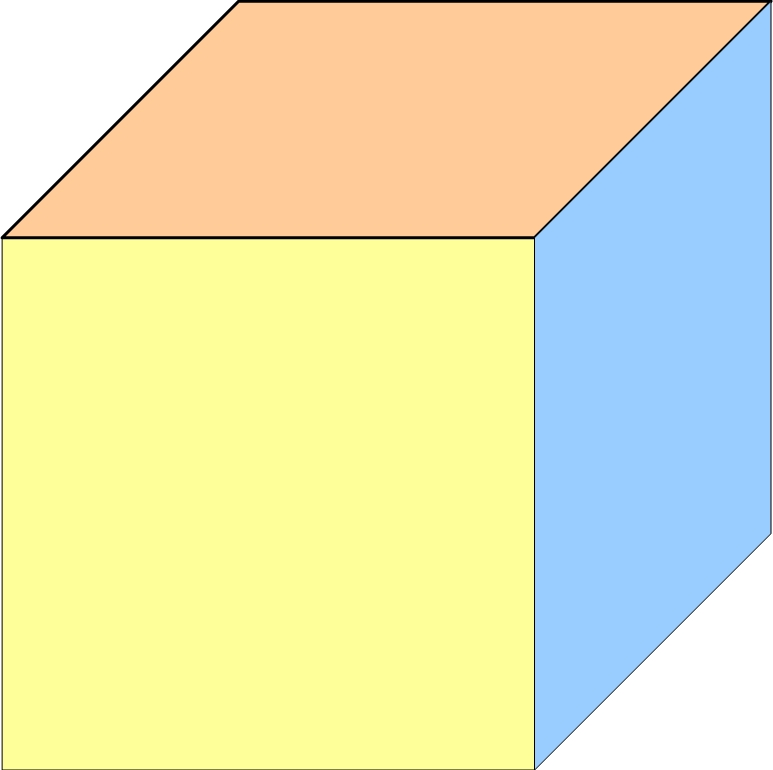
\includegraphics[scale=0.5,bb=0 0 557 554]{./example_fig.jpg}}
 \caption{Caption}
 \label{Label}
\end{figure}
\end{lstlisting}



\begin{figure}[hp]
\centerline{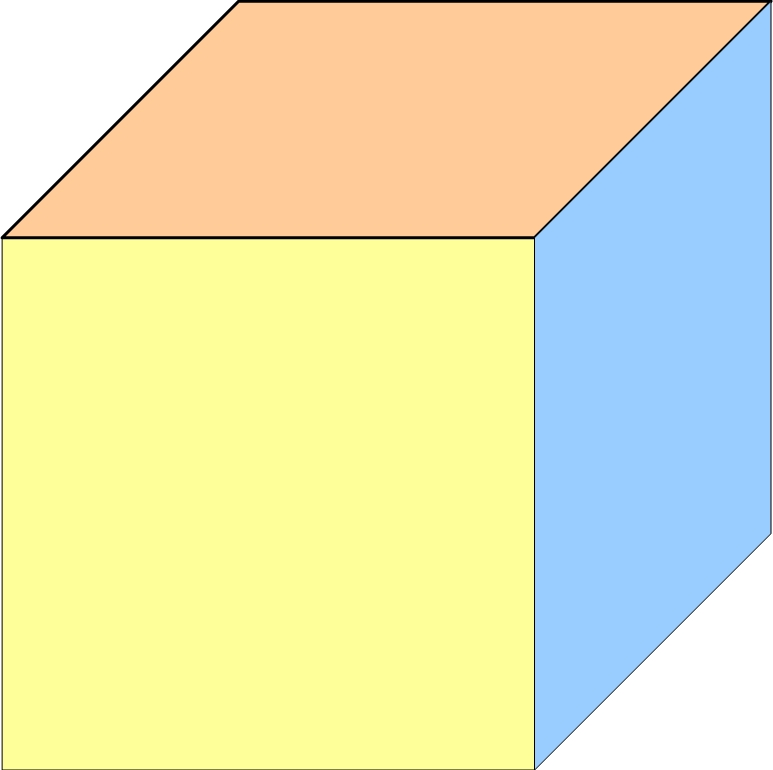
\includegraphics[scale=0.5,bb=0 0 557
554]{./example_fig.jpg}} \caption{This is an example of the
inclusion of a \emph{jpeg-file}} \label{fig:jpeg_ex}
\end{figure}

\begin{figure}[hp]
\centerline{
\includegraphics{./example_fig.eps}} \caption{This is
an example of the inclusion of an \emph{eps-file} with
\emph{includegraphics}} \label{fig:eps_ex_var1}
\end{figure}

\begin{figure}[hp]
\centerline{
\epsfig{file=./example_fig.eps,scale=1.0,angle=0}}
\caption{This is an example of the inclusion of an \emph{eps-file}
with \emph{epsfig}} \label{fig:eps_ex_var2}
\end{figure}
\clearpage

The definition of a table is identically to the definition of a table in the \LaTeX2e standard documentclass \emph{article}.

\begin{table}[hp]
    \begin{center}
    \caption{An example for the inclusion of tables}
    \label{tab:table_ex}
        \begin{tabular}{|c|c|}
        \hline
        Column1 & Columns2\\
        \hline
        \hline
        \ldots & \ldots\\
        \ldots & \ldots\\
        \hline
        \end{tabular}
    \end{center}
\end{table}


\subsection{Special Characters}

An analysis of articles revealed that often symbols like \textreg, \textcright\
and \texttrademark are used. Therefore, the document class \emph{jib} provides
an easy way to insert these symbols. Simply use the commands
\lstinline|\textreg, \textcright| and \lstinline|\texttrademark|. These commands
are part of the \emph{textcomp}-package or are derived from commands of the
\emph{textcomp}-package.


\subsection{Reference Style}

The `vancouver.bst' bibliographic style file (for LaTeX/BibTeX) is generated
with the docstrip utility and modified manually to meet the ``Uniform
Requirements for Manuscripts Submitted to Biomedical Journals'' as published in
N Engl J Med 1997;336:309-315. (also known as the Vancouver style).

This specification may be found on the web page of the International Committe of
Medical Journal Editors:

\url{http://www.icmje.org}

\subsubsection{Copyright Vancouver Style File}

Copyright 2004  Folkert van der Beek

This work may be distributed and/or modified under the conditions of the LaTeX
Project Public License, either version 1.3 of this license or (at your option)
any later version.
The latest version of this license is in
  \url{http://www.latex-project.org/lppl.txt}
and version 1.3 or later is part of all distributions of LaTeX version
2005/12/01 or later.

This work has the LPPL maintenance status `maintained'.

The Current Maintainer of this work is Folkert van der Beek.

More information and also contact info can be found at this website:

\url{https://www.ctan.org/tex-archive/biblio/bibtex/contrib/vancouver?lang=en}


\subsubsection{Usage}

This bibliography style file is intended for texts in ENGLISH
This is a numerical citation style, and as such is standard LaTeX.
It requires no extra package to interface to the main text.
The form of the
 
\begin{lstlisting}
\bibitem
\end{lstlisting}
 

entries is

\begin{lstlisting}
\bibitem{key}...
\end{lstlisting}
  
Usage of 

\begin{lstlisting}
\cite 
\end{lstlisting}

is as follows:

\begin{lstlisting}
\cite{key} ==>>          [#]
\cite[chap. 2]{key} ==>> [#, chap. 2]
\end{lstlisting}
  
where \# is a number determined by the ordering in the reference list.
The order in the reference list is that by which the works were originally
  cited in the text, or that in the database.

To change the reference numbering system from [1] to 1,
put the following code in the preamble:

\begin{lstlisting}
\makeatletter % Reference list option change
\renewcommand\@biblabel[1]{#1} % from [1] to 1
\makeatother %
\end{lstlisting}



%%%%%%%%%%%%%%%%%%%%%%%%%%%%%%%%%%%%%%%%%%%%%%%%%%%%%%%%%%
%
% Bibliography
%
%%%%%%%%%%%%%%%%%%%%%%%%%%%%%%%%%%%%%%%%%%%%%%%%%%%%%%%%%%
\addcontentsline{toc}{section}{References}
\bibliographystyle{vancouver}
\bibliography{jib_references}
\nocite{*}

\end{document}
